% CHAPTER 6: Encoder architecture
\chapter{Encoder Architecture}

I hope that the previous chapters have provided you with a good conceptual understanding of the various components of the encoder architecture of the transformer. In this chapter, we will see how the different components function together to make up the encoder of the transformer. Before proceeding, it will be good to keep in mind the simplified representation of the encoder.
\begin{figure}[H]
    \centering
    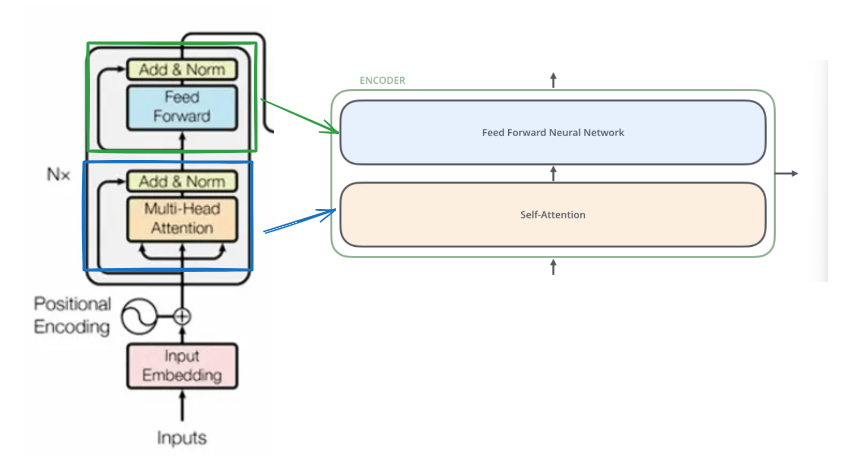
\includegraphics[width=0.75\linewidth]{Encoder/architecture-encoder.png}
    \caption{Encoder architecture of transformer}
\end{figure}

One thing to note is that there is not one, but multiple encoder blocks used in the architecture. In the original paper, the researchers used 6 encoding and decoding blocks. All the blocks have the same design, but have different values of weights in them. Understanding one is sufficient for knowing how all of them work together.

% Input to encoder
\section{Input to the encoder}
Let us consider that we want to pass the sentence \textbf{How are you?} to the transformer. It is first converted into embedding vectors (512 dimensional, as used in the original paper) and then positional encoding is applied. Given below is a schematic diagram of the same.
\begin{figure}[H]
    \centering
    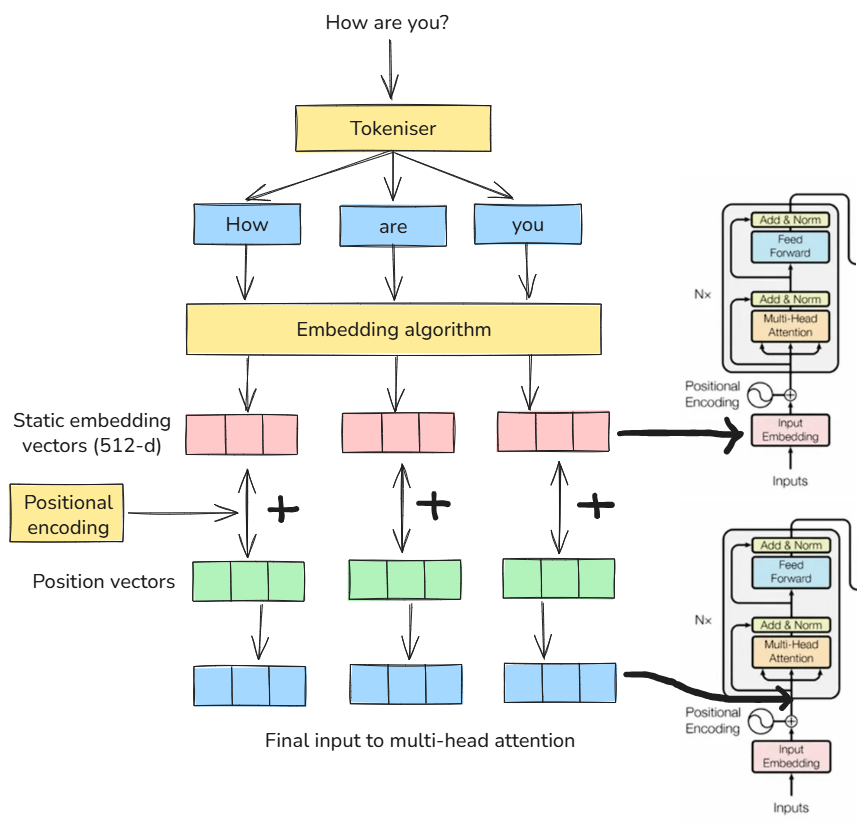
\includegraphics[width=0.75\linewidth]{Encoder/input-pe-encoder.png}
    \caption{Processing of input before going inside the encoder}
\end{figure}

% Multi-head attention and normalisation
\section{Multi-head attention and layer normalization}
The input obtained after positional encoding is passed on to the multi-head attention block. The output from multi-head attention and the input are added and normalized to give the output.
\begin{figure}[H]
    \centering
    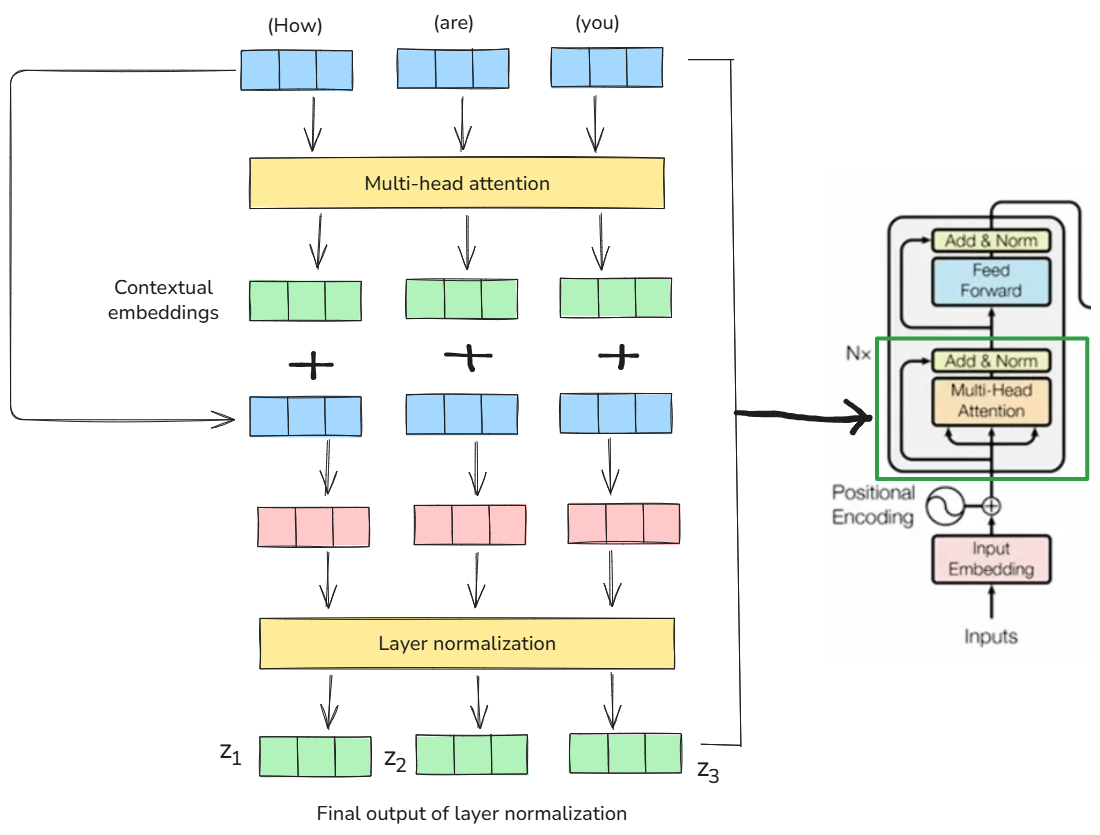
\includegraphics[width=0.75\linewidth]{Encoder/multi-layernorm-encoder.png}
    \caption{Multi-head attention and layer normalization}
\end{figure}

% Feed forward NN
\section{Feed forward neural network (FFNN) and normalization}
The output from multi-head attention are vectors. The number of vectors is same as the number of input tokens. These are stacked up to form a matrix. Input into the FFNN goes in the form of "batches" of a fixed size. The network has:
\begin{enumerate}
    \item \textbf{1 input layer} of 512
    \item \textbf{1 hidden layer} of 2048 neurons (activation function - ReLU)
    \item \textbf{1 output layer} of 512 neurons (activation function - Linear)
\end{enumerate}

This is the same architecture as used by the researchers in the original paper and are adjustable for specific use-cases. The output from the neural network is normalized to get the final output.
\begin{figure}[H]
    \centering
    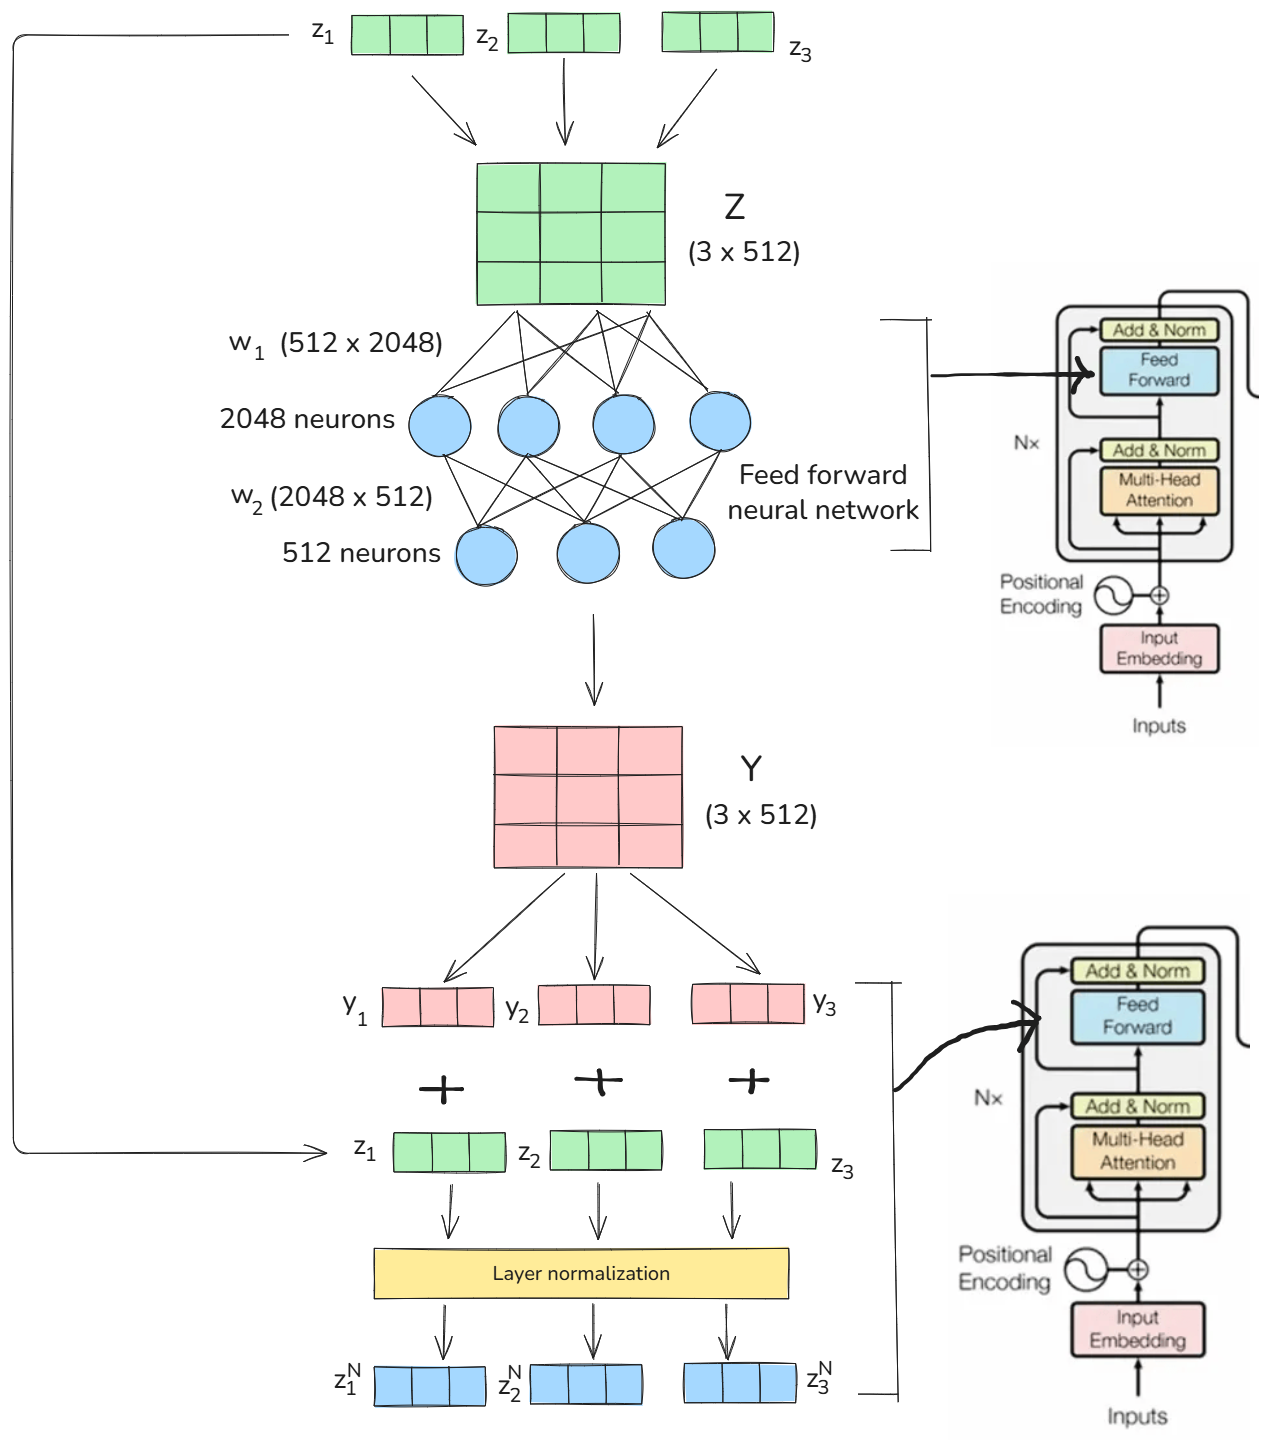
\includegraphics[width=0.75\linewidth]{Encoder/feed-forward-nn-encoder.png}
    \caption{Feed forward NN}
\end{figure}

From the figure,
$$Y = ReLU(Zw_1 + b_1)\,w_2 + b_2$$

where $b_1$ and $b_2$ are the biases of the hidden and output layers respectively and
$$ReLU(z) = max(0, z)$$

The entire encoder architecture can be viewed in this \underline{\href{https://drive.google.com/file/d/1v8-D6W65u3yiwaTBs2UawfwvU7gP4ulE/view?usp=drive_link}{image}}.

% Questions
\section{Some common questions (that do not have definite answers!)}

At this point, you may be having some questions regarding the architecture. Some (I hope most!) of them have been answered below.

\textbf{Why are residual connections used?}\\
This does not have a definite theory mentioned in the original paper, but there are some explanations:
\begin{enumerate}
    \item \textbf{Stabilising the training process:} Since we are sending some part of the input, this prevents the gradients (calculated during backpropagation for updating weights) from becoming too small (preventing \textit{vanishing gradient problem}).
    \item \textbf{Preserving input features:} This preserves the exact features of the input, in case the operation does not provide satisfactory output.
\end{enumerate}

\textbf{Why do we use a feed forward network?}\\
Again, this also does not have a definite answer. The following are proposed as the possible reasons:
\begin{enumerate}
    \item \textbf{Non-linear transformation:} The FFNN adds a layer of complexity by applying non-linear functions to the data representation. This allows the model to learn more intricate (non-linear) patterns in the data.

    \item \textbf{Feature Enhancement:} The FFNN can also be seen as a way to refine the features extracted by the self-attention layer. It can emphasize important features and suppress less relevant ones, making the final output more informative.
\end{enumerate}

\textbf{Why do we use 6 encoder and decoder blocks?}\\
This number was experimentally found out by the researchers to give the best possible output in their case. It can be adjusted in different transformer architectures to check which combination gives the best output.


With this, we have got a clear picture of how the encoder in a transformer works. This covers more than half of our discussion on the working of transformers. From the next chapter, we will focus on the components that make up the decoder part of the transformer. The good thing is that many of the components used in the encoder are also used in the decoder. Hence, our discussion will be a bit easier.